%!TEX root = ./intern_report.tex

\newpage
\subsection{Wave external software tools}
\label{sec:swtools}
\subsubsection{Overview}
\paragraph{}
Working at Wave computing, I was exposed to the use of a lot of software automation tools that are used all over the world in design, development and testing of large scale industrial projects. Working with this expensive software with a crucial part of my internship experience.

The main external software tools used by wave are,
\begin{itemize}
    \item GitLab
    \item Jenkins
    \item Confluence
    \item Jira
    \item Slack
    \item Zoom
\end{itemize}

\paragraph{}
Apart from these software wave computing uses other special software in testing procedures. In general view, working with these expensive software tools is one of the best experiences that I obtained during the internship of six months.

\subsubsection{GitLab}
\paragraph{}
Git is an open source protocol used to manage software code bases collaboratively. A collection of code stored on a git server is called a repository. Users can create 'clones' of the repository on their local computers and edit the code and push the changed code back into the repository. For easier management, users can also create branches in the local clones and make the edits in them, and then merge them back together, as shown in figure \ref{Fig:gitprot}. Git protocol has been successfully adopted and rebranded by a number of companies incluing Github and GitLab.

\begin{figure}[H]
    \centering  
    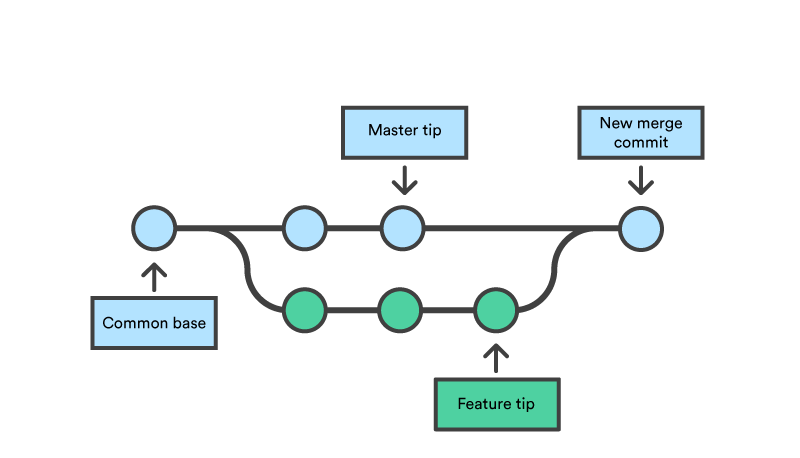
\includegraphics[trim=0cm 0cm 0cm 0cm, clip=true,scale=0.7]{figures/git.png}
    \caption{Git protocol functionality\label{Fig:gitprot}}\vspace{-4mm}
    \end{figure}

\paragraph{}
Wave computing uses GitLab as the main version control software. Since the use of version control in development of software project was not an entirely familiar topic for me I started working with them from scratch. I learnt about the efficient use of such systems and their various advantages in development of software projects. I realized the significance of such systems where developers from scattered everywhere could work according to a centralized plan and develop the same project from different operating from different parts of the world. Apart from that I experienced the advanced techniques used by large development communities in order to track every step of the development of a large scale project. 

\subsubsection{Jenkins}
\paragraph{}
Wave computing uses Jenkins as the test base for their automated testing procedure. Use of Jenkins in testing was an entirely new experience for me. A test run on Jenkins covered up all tests that are needed to be run on any wave flow graph design. After compilation and verification of the functionality of each wave flow graph design I was requested to run a mandatory test done on Jenkins before merging it with the main design of the master. In the event of failure of any of the designs I was assigned to investigate the reasons, rerun tests and make sure that the design was fully functional before engaging it with the main design. 

\begin{figure}[H]
    \centering  
    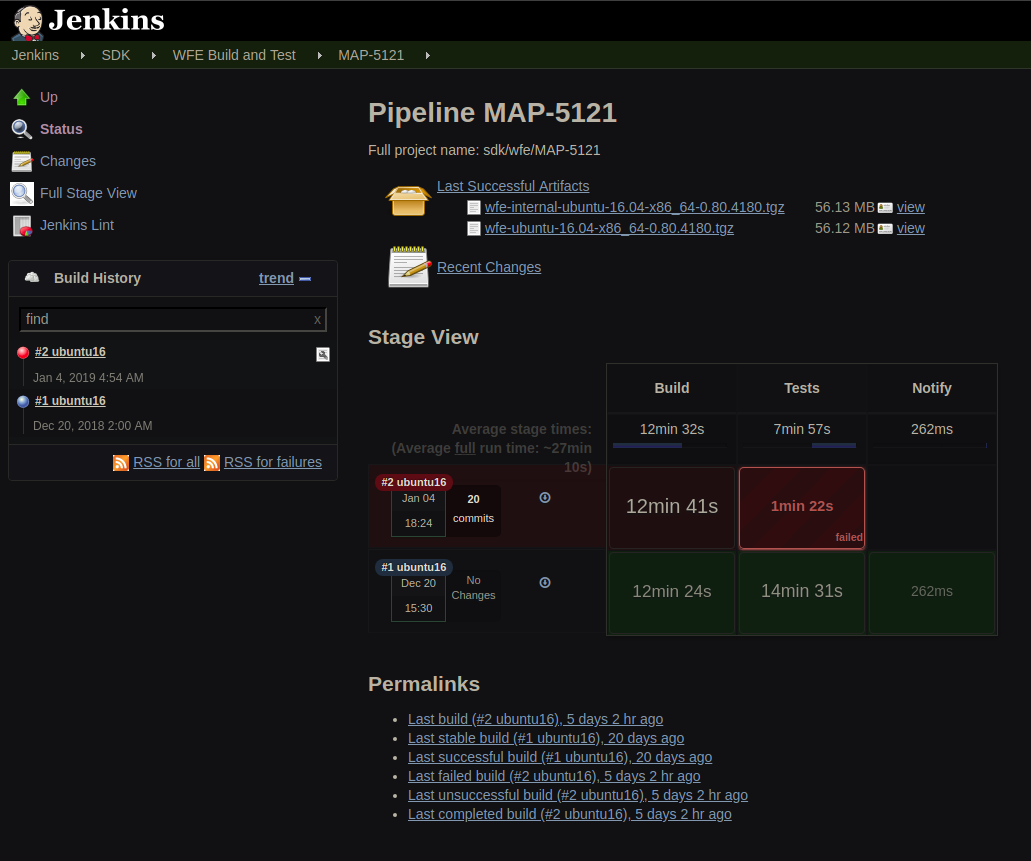
\includegraphics[trim=0cm 0cm 0cm 0cm, clip=true,scale=0.6]{figures/jenkins.png}
    \caption{Jenkins user interface\label{Fig:jenk}}\vspace{-4mm}
    \end{figure}

\paragraph{}
Figure \ref{Fig:jenk} shows Jenkins after a branch had two builds, one that passed the tests (Green) and one that failed in the middle (Red). It also shows the branch name, build/test times and that it belongs to the WFE repository.

\subsubsection{Confluence}
\paragraph{}
Documentation of all Wave Computing related details are maintained in a Confluence page. I witnessed the importance of documentation while exploring various archives of Wave design development tools. I realized the downside to apparent dissatisfaction among the developers in maintaining properly updated archives of software development projects. I ran into a number of troubles due to outdated or insufficiently developed documents, specially about the DMA engine of the WFGsim. This contained a number of conflicted documents scattered around the Confluence site. However, I managed to gather these documents and extract a final definition of the DMA engine and build a replacement on my own.

\subsubsection{Jira}
\paragraph{}
Jira is the official issue tracker for Wave Computing team. Any issues, bugs, improvements or changes to the wave design flow are recorded as tasks in Jira. Resolving these tasks can be assigned to any of the design individuals of the wave computing team. Usually the tasks come with supervisors and senior consultants in charge of completion of it. Any changes or developments to that is updated to the Jira so that everyone can access the information and get an idea about the current status of the Wave design tools. It is a very convenient way of managing projects and deciding on the development of software project carried out with collaborators from all over the world. 

\subsubsection{Slack}
\paragraph{}
All the text based communication within Wave is carried out via Slack. It is like a normal instant messaging app that we have for our normal usage (Eg. Whatsapp) but has a lot of Enterprise focused features. It has the capability to separate work related content on channels, organize notifications on priority and enhanced search/organization capabilities. It is also available in almost every platform, mobile, windows, linux or web, making it perfect for a company that uses many platforms on their computing systems.

\subsubsection{Zoom}
While slack handles texting, zoom is the video calling platform of Wave. As the management of the company is overseas, high quality video calling is essential for Wave. Zoom provides this with their highly optimized VoIP technologies. Even when the internet connection is poor, which is a common problem in Sri Lanka, Zoom can maintain an acceptable link over it. 

\subsubsection{Usage of tools in the SDK verification flow}
\paragraph{}
The Wave SDK is a massive piece of software that has all the necessary features for writing a program for the DPU and testing it in a proper,thorough manner. This whole kit is still under construction and new edits need to be added to the code everyday but this should be done in a manner that does not break the existing code. This is done via a clever combination of GitLab and Jenkins as illustrated in Figure~\ref{Fig:build}

\begin{figure}[H]
    \centering  
    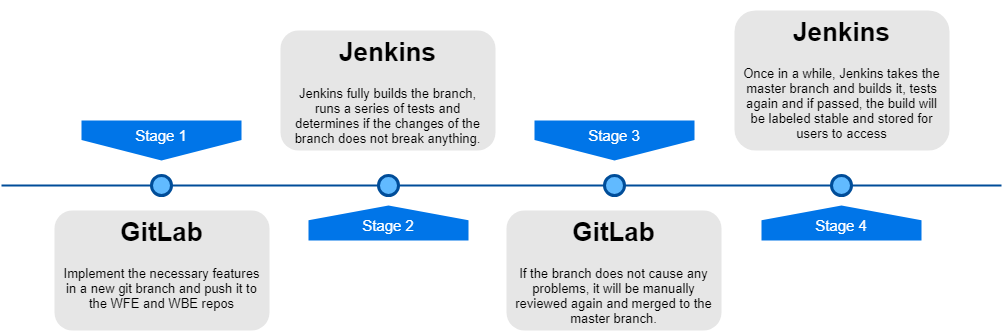
\includegraphics[trim=0cm 0cm 0cm 0cm, clip=true,scale=0.4]{figures/build.png}
    \caption{Wave SDK build flow\label{Fig:build}}\vspace{-4mm}
    \end{figure}